\chapter{Marco de Referencia}

 Desde finales del siglo pasado, los avances tecnológicos en la miniaturización de la electrónica y los componentes mecánicos han allanado el camino para la creación y desarrollo de objetos voladores de pequeñas dimensiones, tales como aviones y helicópteros, los cuales están adquiriendo cada vez más habilidades para realizar vuelos de forma autónoma. Estos dispositivos son popularmente conocidos como drones, un término derivado del inglés \say{abejorros}, y se consideran máquinas voladoras autónomas o semi-autónomas capaces de llevar a cabo misiones de vuelo. En el ámbito internacional, se les conoce como UAVs del ingles \say{Unmanned Aerial Vehicles}, y representan una tecnología compleja cuyo control presenta desafíos, dado que sus características aerodinámicas son similares a las de las aeronaves convencionales \cite{eisenbeiss2004mini}.

El estudio de estos dispositivos despierta un gran interés debido a su versatilidad y capacidad de maniobra, lo que les permite llevar a cabo una amplia gama de tareas en diversas aplicaciones, tales como el uso civil, militar y aeroespacial \cite{nawaz2019applications, shakhatreh2019unmanned, xiaoning2020analysis}. En la figura \ref{fig1_aplicacion_UAV}, se presenta una clasificación detallada de las aplicaciones más importantes de los UAVs.

\begin{figure}[H]
    \centering
    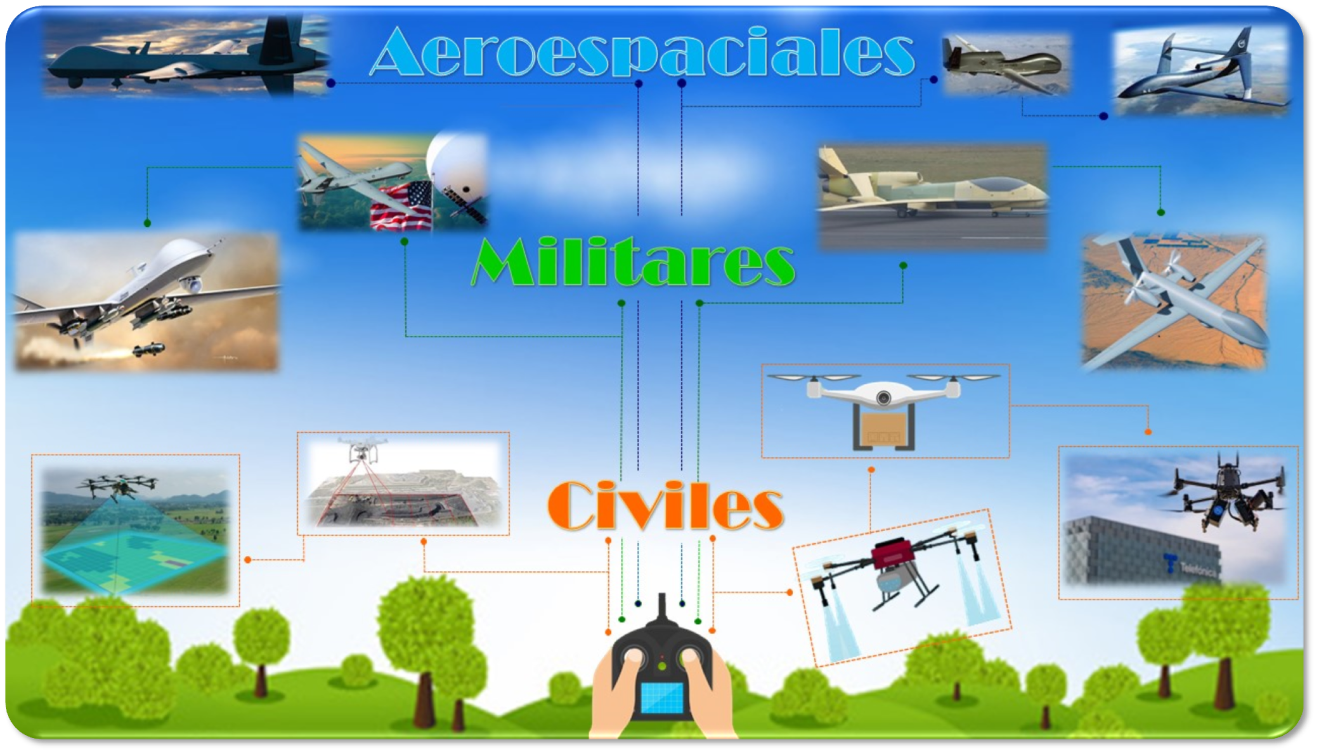
\includegraphics[width=16cm, height=7.5cm]{imagenes/Aplicaciones_UAV.png}
    \caption{Áreas de aplicación UAVS.}
    \label{fig1_aplicacion_UAV}
\end{figure}

\section{Antecedentes.}

Los drones han atraído la atención de la comunidad investigadora que trabaja tanto en el campo militar como en el civil, con una gran cantidad de usos que han sido propuestos por los grupos de investigación, debido a sus características como capacidad y configuraciones, donde el helicóptero de cuatro rotores tiene el mayor número de citas en la literatura de control y ha sido ampliamente investigado para pruebas tanto en interiores como en exteriores . 

\section{Objetivo General}
\textbf{}
\section{Objetivos Especificos}
\begin{enumerate}
\item Recolectar y organizar conjuntos de datos públicos internacionales sobre calidad del aire, variables meteorológicas y factores geoespaciales. 
\item Explorar y analizar las principales tendencias, correlaciones y patrones de comportamiento entre los contaminantes atmosféricos y las variables ambientales, utilizando técnicas de análisis exploratorio de datos.

\end{enumerate}

\section{Alcance}
El proyecto comprenderá el diseño, desarrollo y validación de una aplicación web para la gestión de recursos materiales y de incidencias de mantenimiento e infraestructura en un plantel universitario. Su organización seguirá la arquitectura Modelo–Vista–Controlador (MVC), con Laravel y una base de datos MariaDB. El acceso se realizará mediante cuentas de correo institucional y permisos diferenciados para solicitantes, coordinación, personal técnico y personal de almacén; la administración de usuarios y roles quedará reservada al personal autorizado.
El sistema contemplará el registro de fallas asociadas a edificios y espacios del plantel, con descripción y evidencia fotográfica; la consulta y el seguimiento de los reportes; y su revisión por parte de coordinación. Se incluirán mecanismos para prevenir reportes repetidos y agrupar aquellos que correspondan a una misma incidencia, así como la asignación de técnicos considerando especialidad y turno y la autorización de trabajos que lo requieran por su costo o riesgo.
La gestión operativa abarcará las órdenes de trabajo, el registro de tareas y estados de atención, la solicitud y entrega de materiales, las entradas y salidas de inventario y la consulta de existencias. Las operaciones relevantes se registrarán en bitácora para relacionar reportes, responsables, movimientos de materiales y evidencias de cierre. El cierre de una orden contemplará la comprobación de tareas y el registro de evidencia del trabajo realizado.
La entrega incluirá la documentación técnica y de uso, el modelo de base de datos y las pruebas funcionales, de seguridad y de flujo por rol necesarias para demostrar el proceso de atención de una incidencia. Las funciones descritas constituyen el alcance previsto del proyecto y su cumplimiento se verificará durante las pruebas.


\section{Limitación}
\begin{enumerate}
\item \textbf{Cobertura institucional.} La primera versión se delimitará a un plantel universitario y a los edificios, espacios, usuarios y materiales incorporados a sus catálogos. No se contempla la administración centralizada de múltiples instituciones.

\item \textbf{Entorno de operación.} El uso del sistema dependerá de la disponibilidad de un servidor con PHP y Laravel, una base de datos MariaDB, almacenamiento para las evidencias y acceso a la red desde un navegador compatible. No se contempla una aplicación móvil nativa ni el registro y la sincronización de operaciones sin conexión.

\item \textbf{Dependencia de los datos y de la operación humana.} La calidad del seguimiento dependerá de la captura correcta y oportuna de reportes, asignaciones, movimientos y evidencias por parte de los usuarios autorizados. La identificación de posibles duplicados requerirá revisión de coordinación; el sistema no garantizará la detección automática de todas las incidencias repetidas.

\item \textbf{Integraciones y procesos externos.} No se incluyen integraciones con sistemas institucionales externos, compras, pagos, contabilidad, dispositivos biométricos ni firma electrónica certificada. El control de almacén se enfocará en existencias y movimientos vinculados con la atención de incidencias; no abarcará la gestión completa del ciclo de vida de los activos.

\item \textbf{Validación y tiempos de atención.} Las pruebas se efectuarán con los recursos y escenarios disponibles durante el desarrollo académico. Los resultados de rendimiento se limitarán al entorno y a la carga evaluados. La aplicación apoyará la coordinación y el seguimiento, pero no garantizará un plazo fijo de reparación, ya que este dependerá de la disponibilidad de personal, materiales y autorizaciones.
\end{enumerate}


\section{Problemática}


\section{Justificación}

